\chapter{Appendix: Physical Pion Masses}
\label{ch:appendix:physical:pions}

\readit{0}

%\worktodo{short paragraph leading to plot}

This chapter should give rough indication of the variance reduction when lowering the ensemble pion mass toward its physical value.
We investigated two lattices \cref{tab:pion:ensembles}, which differ only in their respective pion masses.
Lattice extents and spacings are equal.

\begin{table}[t]
\centering
\begin{tabular}{cccc}
\toprule
{ensemble}&
{$L_0 \times L^3$} &
{Pion mass [MeV]} &
{$L$ ($\mathrm{fm}$)} \\
\midrule
G7 & $128 \times 64^3$ & 270 & 4.2 \\
G8 & $128 \times 64^3$ & 180 & 4.2 \\
\bottomrule
\end{tabular}
\caption{\label{tab:pion:ensembles}%
Ensembles used in \cref{fig:var:vs:pion:mass}.
The lattice extent, denoted by $L$, indicates the spatial box extents, $L = L_1 = L_2 = L_3$ and $L_0 = 2L$.
Both lattices have the same lattice extents and lattice spacing of $a = 0.0658(10)$ fm with $\Nf=2$ $\bigO(a)$-improved Wilson fermions with lattice coupling $\beta=5.3$ and $c_\mathrm{sw} = 1.90952$~\cite{online:cls,Jansen:1998mx}.
G8 has been generated by the CLS initiative~\cite{online:cls}, while the other is from the numerical study \cref{tab:mglma:ensembles}.
We used $\cNc=50$ low modes on both lattices and the same multigrid setup.
}
\end{table}

When looking at the variance contribution of their \Ln{0} terms in \cref{fig:var:vs:pion:mass}, we see no noticeable change when going from $m_{\pi} \approx $ \u{270}{\MeV} to $m_{\pi} \approx $ \u{180}{\MeV}.
Although, this is not a conclusive study with only two datapoints and the lower pion mass still not at the physical values of $m_{\pi} \approx $ \u{135}{\MeV}, it nevertheless gives a rough indication that the method scales well, also on lower pion masses.

Furthermore, one expects the property of local coherence of low modes to be even more pronounced on physical pion mass ensembles~\cite{Luescher2007}.

\begin{figure}
\centering
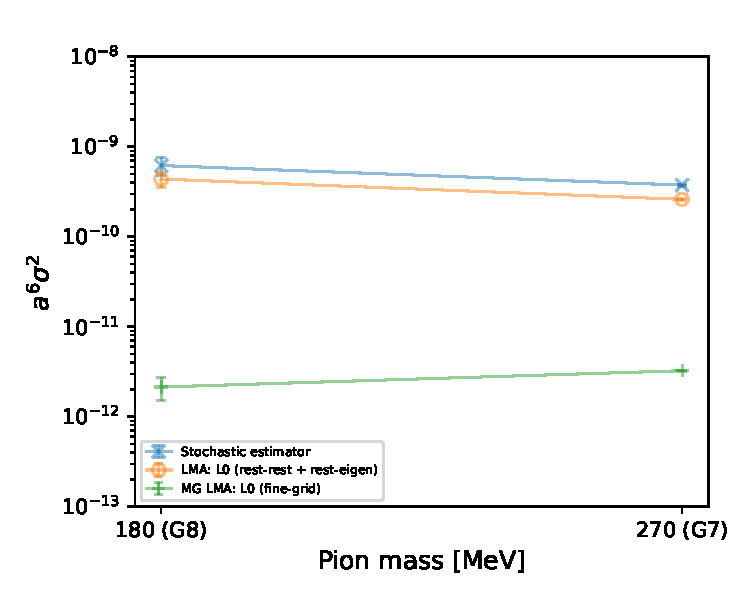
\includegraphics[width=0.6\linewidth]{\dir/img/var_vs_pion_mass}
\caption{
Absolute total variance \cref{eq:abs:variance} of the \Ln{0} term vs. the ensemble pion mass.
The \Ln{0} variance contribution of LMA (yellow) and MG LMA (green) do not change within their error bars.
The blue solid line represents the pure stochastic estimator without any deflation.
}
\label{fig:var:vs:pion:mass}
\end{figure}
